\chapter{Metodologi}

Pada bab ini menjelaskan mengenai metodologi yang digunakan selama pengerjaan tugas akhir.

\begin{figure}[H]
	\begin{centering}
		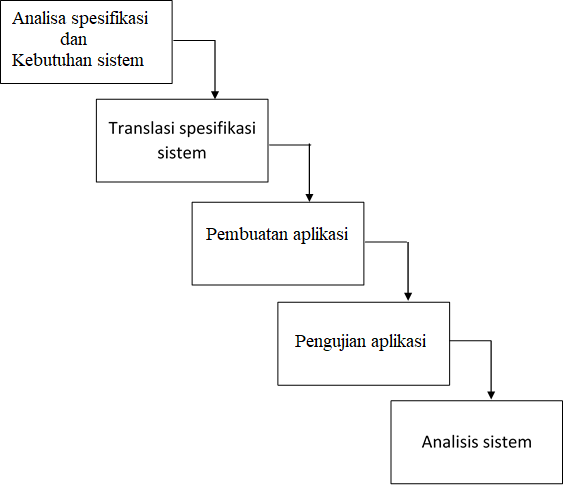
\includegraphics[scale=0.7]{metodologi_proposal}
		
		\caption{Contoh metodologi.}
	\end{centering}
\end{figure}

\section{Analisa spesifikasi dan Kebutuhan sistem}

Data didapatkan dari . . . .

\section{Translasi spesifikasi sistem}

Data yang telah didapatkan akan ditranslasi dalam  . . . .

\section{Pembuatan aplikasi}

Data yang telah didapatkan akan diubah dalam model formal . . . .

\section{Pengujian aplikasi}

Model formal yang telah dibuatkan akan diverifikasi menggunakan . . . .

\section{Analisis sistem}

Hasil verifikasi akan dianalisis . . . .